\chapter{Pengantar Fisika Kuantum}\label{ch:b1:quantum-introduction}

Sinarilah sebuah logam yang bersih dengan cahaya ultraungu dan elektron
terlontar keluar seketika, dengan energi yang bergantung pada warna cahayanya dan
sama sekali tak pada terangnya; sinarilah dengan cahaya merah dan tak ada yang keluar
betapa pun terang lampunya. Kirimkanlah elektron satu demi satu lewat dua celah dan
mereka mendarat sebagai titik, masing-masing di satu tempat --- dan titik-titiknya
menumpuk, setelah beribu-ribu, menjadi rumbai sebuah gelombang. Kedua kenyataan itu
tak muat dalam fisika dua puluh sembilan bab pertama. Bab terakhir ini memperkenalkan
gagasan yang memang memuatnya: cahaya datang dalam kuanta, yaitu foton; materi memiliki
panjang gelombang; yang merambat adalah sebuah \omterm{def:b1:wave-propagation:signal}{amplitudo} yang kuadratnya sebuah
peluang; kedudukan dan momentum tak dapat tajam dua-duanya; dan sebuah partikel
terkurung hanya dapat memiliki energi tertentu --- dan itulah sebabnya atom
berukuran, spektrum bergaris, dan sebutir semikonduktor selebar beberapa
nanometer berpendar dalam warna yang ditetapkan garis tengahnya.

\section{Foton}

\begin{theorem}[Hubungan Planck--Einstein]\label{thm:b1:quantum-introduction:photon}
\index{foton}\index{tetapan Planck}
Cahaya berfrekuensi $\nu$ dan berpanjang gelombang $\lambda$ bertukar energi dengan
materi hanya dalam kuanta, yaitu \emph{foton}, yang berenergi dan bermomentum
\[
E = h\nu = \frac{hc}{\lambda} , \qquad p = \frac{h}{\lambda} = \frac{E}{c} ,
\]
dengan \emph{\omterm{thm:b1:quantum-introduction:photon}{tetapan Planck}} $h = \qty{6.626e-34}{J.s}$ ($\hbar = h/2\pi =
\qty{1.055e-34}{J.s}$). Berguna: $hc = \qty{1240}{eV.nm}$ --- sebuah foton
\qty{620}{nm} mengemban \qty{2}{eV}.
\end{theorem}
\admitted

\begin{proposition}[Efek fotolistrik]\label{prop:b1:quantum-introduction:photoelectric}
\index{efek fotolistrik}\index{fungsi kerja}\index{potensial henti}
Cahaya yang jatuh pada sebuah logam dengan \emph{\omterm{prop:b1:quantum-introduction:photoelectric}{fungsi kerja}} $W$ (energi yang
mengikat elektronnya yang paling lemah terikat, beberapa eV) melontarkan elektron
berenergi kinetik maksimal
\[
E_{k,\max} = h\nu - W ,
\]
jadi hanya di atas \emph{ambang} $\nu_0 = W/h$, seketika, dengan
energi yang tak bergantung pada intensitasnya; intensitasnya menetapkan
\emph{banyaknya} elektron tiap sekon. Yang disebut \emph{\omterm{prop:b1:quantum-introduction:photoelectric}{potensial henti}}
$V_s$, yang tepat meniadakan arusnya, mengukur $E_{k,\max} = eV_s$, dan
grafik $V_s$ terhadap $\nu$ berupa garis lurus berkemiringan $h/e$ --- begitulah
Millikan mengukur $h$.
\end{proposition}

\begin{proof}
Tiap fotonnya diserap oleh satu elektron, yang paling banter menyimpan $h\nu - W$;
sebuah gelombang akan menyalurkan energi secara sinambung kepada setiap elektronnya,
energinya akan tumbuh bersama intensitasnya, dan cahaya yang lemah akan perlu berjam-jam untuk
menumpuk $W$ pada satu atom (\cref{pb:b1:quantum-introduction:1}) ---
tak satu pun teramati. Tafsiran Einstein (1905) diterima tanpa bukti
sebagai hukumnya.
\end{proof}

\begin{omfigure}
\begin{tikzpicture}[font=\small, x=1cm, y=1cm, >=Stealth]
  % apparatus
  \draw[fill=omExo!25, draw=omExo, thick] (-2.2,-1.2) rectangle (-1.7,1.2); \node[font=\footnotesize] at (-1.95,-1.5) {katode};
  \draw[omThm, thick] (1.7,-1.2) -- (1.7,1.2); \node[font=\footnotesize] at (1.7,-1.5) {anode};
  \foreach \y in {0.6,0.2,-0.2} \draw[omProp, ->, decorate, decoration={snake, amplitude=1.5pt, segment length=4pt, post length=3pt}] (-3.8,\y+0.6) -- (-2.25,\y);
  \node[omProp, font=\footnotesize] at (-3.6,1.55) {cahaya, $\nu$};
  \foreach \y in {0.7,0,-0.7} \draw[omDef, ->] (-1.65,\y) -- (0.4,\y);
  \node[omDef, font=\footnotesize] at (0,1.0) {$E_k \leq h\nu - W$};
  \draw (-1.95,-1.2) -- (-1.95,-2.2) -- (1.7,-2.2) -- (1.7,-1.2);
  \draw[fill=white] (-0.6,-2.45) rectangle (0.4,-1.95); \node[font=\footnotesize] at (-0.1,-2.2) {$V_s$};
  \node[font=\footnotesize] at (-0.1,-2.75) {anode ditahan pada $-V_s$: arusnya tepat nol};
\end{tikzpicture}\hfill
\begin{tikzpicture}
\begin{axis}[omaxis, axis x line=bottom, axis y line=left, width=7.4cm, height=5.4cm,
    xlabel={$\nu$ ($10^{14}$ Hz)}, ylabel={$V_s$ (V)},
    xlabel style={at={(axis description cs:1.0,0.0)}, anchor=north east, yshift=-10pt},
    xmin=0, xmax=12.5, ymin=0, ymax=3, xtick={2,4,...,12}, ytick={1,2,3}, samples=2, clip=false]
  \addplot[omDef, thick, domain=5.32:12] {0.4136*x-2.2};
  \addplot[only marks, mark=*, mark size=1.6pt, omThm] coordinates {(6,0.30) (7,0.69) (8,1.13) (9,1.50) (11,2.36)};
  \addplot[omDef, dashed, thin, domain=3.6:5.32] {0.4136*x-2.2};
  \node[font=\footnotesize, omDef, anchor=east] at (axis cs:3.4,-0.6) {pintasan $-W/e$};
  \node[font=\footnotesize, anchor=south] at (axis cs:5.32,0.05) {$\nu_0$};
  \node[font=\footnotesize, omDef, anchor=west] at (axis cs:8.4,0.9) {kemiringan $h/e$};
\end{axis}
\end{tikzpicture}

{\small Kiri: sel fotolistriknya --- cahaya membebaskan elektron dari
katodenya; \omterm{def:b1:dc-circuits:voltage}{tegangan} balik $V_s$ yang tepat cukup untuk menghentikannya mengukur
energi maksimalnya. Kanan: \omterm{prop:b1:quantum-introduction:photoelectric}{potensial henti} terhadap frekuensi
berupa garis lurus bagi setiap logam, berkemiringan $h/e$; pintasannya memberi
\omterm{prop:b1:quantum-introduction:photoelectric}{fungsi kerjanya}, ambangnya memberi frekuensi minimumnya.}
\end{omfigure}

\begin{example}[Orde besarnya]\label{ex:b1:quantum-introduction:orders}
Sebuah foton tampak: \qty{2}{eV}; sebuah foton sinar-X \qty{0.1}{nm}: \qty{12}{keV};
sebuah foton radio pada \qty{100}{MHz}: \qty{4e-7}{eV}. Sebuah laser merah \qty{1}{mW}
memancarkan $10^{-3}/(3.1 \times 10^{-19}) = 3 \times 10^{15}$ foton tiap sekon;
sebuah antena radio yang memungut \qty{1}{pW} pada \qty{100}{MHz} menerima $10^{13}$
tiap sekon --- begitu banyak, begitu kecil, sehingga pemerian gelombangnya tepat
untuk keperluan apa pun; sebaliknya \omterm{def:b1:optical-instruments:eye}{mata} dapat mencatat sebuah kilatan
seratus foton. Sifat kuantum cahaya tampak ketika fotonnya
sedikit atau bertenaga: sel fotolistrik, pendeteksi sinar-X, butiran
sebuah foto yang samar.
\end{example}

\begin{remark}[Hamburan Compton]\label{rem:b1:quantum-introduction:compton}
\index{hamburan Compton}
Sebuah foton yang memantul dari elektron bebas memindahkan momentum seperti
bola bilyar: panjang gelombangnya tumbuh sebesar $\Delta\lambda = \frac{h}{m_ec}(1 -
\cos\theta)$, dengan $h/m_ec = \qty{2.43}{pm}$ (diterima tanpa bukti --- sebuah tumbukan
relativistik, Tahun ke-2). Tak terlihat bagi cahaya ($\Delta\lambda/\lambda \sim 10^{-5}$),
ia menjadi efek $20\%$ bagi sinar-X, dan menjadi percobaan yang meyakinkan
kaum peragu (1923) bahwa foton mengemban momentum $h/\lambda$.
\end{remark}

\section{Gelombang materi}

\begin{theorem}[de Broglie]\label{thm:b1:quantum-introduction:debroglie}
\index{panjang gelombang de Broglie}\index{gelombang materi}
Sebuah partikel bermomentum $p$ merambat sebagai gelombang berpanjang gelombang
\[
\lambda = \frac{h}{p} ,
\]
dan sejalan dengan itu memperlihatkan difraksi dan interferensi: elektron pada
sebuah kristal (Davisson dan Germer, 1927), lewat dua celah (Jönsson, 1961),
neutron, atom, dan molekul beratom karbon enam puluh. Bagi sebuah elektron
yang dipercepat oleh $U$, $\lambda = h/\sqrt{2m_eeU} = \qty{1.23}{nm}/\sqrt{U/\unit{V}}$.
\end{theorem}
\admitted

\begin{example}[Mengapa kita tak pernah melihatnya]\label{ex:b1:quantum-introduction:wavelengths}
Sebuah elektron \qty{100}{eV}: $\lambda = \qty{0.12}{nm}$, yaitu jarak antara
atom dalam sebuah kristal --- karena itulah difraksinya, dan \omterm{def:b1:optical-instruments:microscope}{mikroskop}
elektronnya. Sebuah neutron termal (\qty{0.025}{eV}): \qty{0.18}{nm}. Sebuah bola
\qty{1}{g} pada \qty{1}{m/s}: $\lambda = \qty{7e-31}{m}$, $10^{20}$ kali
lebih kecil daripada sebuah inti: tak ada celah, tak ada kristal yang dapat mendifraksikannya.
Sifat \omterm{thm:b1:quantum-introduction:debroglie}{gelombang materi} bersifat semesta; panjang gelombangnyalah yang membuatnya
terlihat hanya bagi yang ringan dan yang lambat.
\end{example}

\begin{proposition}[Partikel tunggal membangun rumbainya]\label{prop:b1:quantum-introduction:buildup}
\index{dualitas gelombang--partikel}
Elektron yang dikirim satu per satu lewat dua celah (Tonomura, 1989) masing-masing
membuat satu titik pada layarnya, di tempat yang tak dapat diramalkan;
titiknya menumpuk menjadi pola interferensi dua celah sebuah gelombang
berpanjang gelombang $h/p$. Menutup salah satu celahnya menghapus rumbainya --- polanya
bukan dibuat oleh elektron yang berinterferensi satu sama lain, melainkan oleh
gelombang tiap elektron yang lewat kedua celahnya. Mendeteksi lewat celah mana
sebuah partikel pergi juga menghapus rumbainya.
\end{proposition}
\admitted

\begin{omfigure}
\begin{tikzpicture}[font=\small, x=1cm, y=1cm]
  \begin{scope}
    \draw (-3.2,0) rectangle (3.2,1.3);
    \foreach \x/\y in {-0.42/0.13, -0.48/1.04, 1.15/0.56, 0.55/0.59, 0.60/0.75, -0.69/0.53, -0.22/0.63, 0.11/0.48, 0.98/1.01, 0.53/1.14, 0.15/0.07, 0.79/0.66, 0.45/0.89, -1.25/0.96, 0.00/0.26, -3.08/0.35, -0.16/1.17, 1.20/1.23, -0.61/0.47, -1.22/0.48, -1.91/0.66, 0.03/1.05, 1.17/0.88, -0.07/0.05, 0.75/0.82, -1.25/0.73, 1.23/0.86, 0.11/0.61, 3.06/1.17, -1.18/1.06, -0.46/0.38, 0.07/0.28, 0.15/0.50, 0.53/0.52, 0.65/0.06, 1.12/0.55, 1.07/1.16, 1.06/1.19, -1.17/0.38, -0.73/0.35, -0.04/1.16, -1.62/0.13, -0.53/0.79, 0.05/0.33, 0.53/1.17, 0.62/0.79, 1.14/0.27, -1.20/0.73, -0.49/1.03, 0.11/0.51, 0.64/0.71, -0.48/0.84, -0.07/0.33, -0.17/0.18, 0.07/0.10, 0.07/0.12, -0.78/1.19, -0.05/1.20, 0.04/0.43, 1.15/1.12} \fill[omDef] (\x,\y) circle (1.1pt);
    \node[font=\footnotesize] at (0,-0.35) {$60$ elektron};
  \end{scope}
  \begin{scope}[yshift=-2.4cm]
    \draw (-3.2,0) rectangle (3.2,1.3);
    \foreach \x/\y in {-0.42/0.13, -0.48/1.04, 1.15/0.56, 0.55/0.59, 0.60/0.75, -0.69/0.53, -0.22/0.63, 0.11/0.48, 0.98/1.01, 0.53/1.14, 0.15/0.07, 0.79/0.66, 0.45/0.89, -1.25/0.96, 0.00/0.26, -3.08/0.35, -0.16/1.17, 1.20/1.23, -0.61/0.47, -1.22/0.48, -1.91/0.66, 0.03/1.05, 1.17/0.88, -0.07/0.05, 0.75/0.82, -1.25/0.73, 1.23/0.86, 0.11/0.61, 3.06/1.17, -1.18/1.06, -0.46/0.38, 0.07/0.28, 0.15/0.50, 0.53/0.52, 0.65/0.06, 1.12/0.55, 1.07/1.16, 1.06/1.19, -1.17/0.38, -0.73/0.35, -0.04/1.16, -1.62/0.13, -0.53/0.79, 0.05/0.33, 0.53/1.17, 0.62/0.79, 1.14/0.27, -1.20/0.73, -0.49/1.03, 0.11/0.51, 0.64/0.71, -0.48/0.84, -0.07/0.33, -0.17/0.18, 0.07/0.10, 0.07/0.12, -0.78/1.19, -0.05/1.20, 0.04/0.43, 1.15/1.120} \fill[omDef] (\x,\y) circle (1.1pt);
    \node[font=\footnotesize] at (0,-0.35) {$600$ elektron};
  \end{scope}
  \begin{scope}[yshift=-4.6cm]
    \draw (-3.2,0) rectangle (3.2,1.3);
    \foreach \x/\y in {-0.02/0.94, 1.23/0.49, -1.77/0.11, 0.08/1.17, 0.58/0.98, -0.45/0.37, -1.29/0.96, -0.08/0.50, 0.27/1.07, -0.57/0.51, -0.57/0.28, -0.12/0.06, -0.00/0.62, 0.20/0.90, -0.01/0.81, -0.08/1.16, 0.57/0.90, -1.18/0.87, 0.47/0.79, 0.15/0.87, -0.77/1.01, -0.58/0.94, 0.06/1.13, 0.67/0.72, 1.29/0.61, 0.75/0.17, 1.23/0.09, -0.76/1.08, -1.29/0.68, -0.14/0.59, -1.13/0.63, 0.56/0.63, 0.13/0.95, 0.61/0.32, 0.05/0.24, -1.19/1.21, -0.68/0.95, 0.08/0.95, -1.25/0.14, -0.00/0.97, 0.46/1.23, -0.01/0.65, -0.49/0.26, 1.21/0.40, 0.62/1.16, -1.13/0.75, -0.47/0.32, 1.05/0.84, 0.73/0.44, 1.35/0.14, -0.07/0.11, -0.63/0.53, 0.02/0.24, 0.53/0.36, 0.35/0.73, 0.02/0.28, 0.63/1.12, 0.50/0.61, -0.21/0.94, -0.06/0.11, -0.09/1.09, 1.15/1.24, 1.06/0.65, 0.62/1.07, 0.74/0.41, -0.09/0.10, 0.75/0.06, -1.06/0.43, -0.55/0.75, 0.68/1.23, 0.06/1.07, 1.37/0.27, 0.48/0.42, -0.45/0.66, 1.22/0.12, 0.55/0.08, 1.17/0.85, 0.11/1.22, -0.13/0.86, 0.15/0.26, -0.55/0.94, 0.10/0.53, 1.26/0.83, -0.79/0.40, -0.04/0.23, 1.21/0.36, -0.14/0.08, -1.27/0.75, -1.29/0.23, 3.02/0.76, 0.62/1.20, 1.26/0.22, -1.16/0.83, -1.03/0.62, -0.02/1.12, -2.97/0.76, 0.12/0.98, -0.40/0.70, -0.57/0.09, -0.03/0.54, 1.74/0.33, 0.60/0.33, -0.61/0.36, -1.08/1.24, -0.58/0.49, 0.52/0.54, -1.08/1.07, 0.48/0.39, 3.01/0.59, 0.14/1.20, -0.75/0.07, -0.42/1.16, -1.16/0.68, 0.15/0.74, -0.12/0.86, 1.37/0.15, 0.72/0.66, -0.60/0.62, 0.48/0.87, -0.63/0.14, 1.88/0.48, 2.91/0.09, 1.77/1.19, -0.71/1.10, -1.77/1.18, -1.00/0.55, -1.21/0.47, 0.04/1.13, -1.31/0.21, -1.39/0.24, -0.77/0.87, -0.12/0.70, -1.31/0.75, -0.02/0.99, 0.70/1.21, -0.51/0.27, 1.17/0.97, -0.09/0.65, -1.29/0.65, 0.58/0.32, 0.61/0.71, -0.54/1.20, -0.02/0.41, -1.11/0.60, 0.63/0.91, -0.02/0.47, 0.63/0.36, -0.00/0.16, -0.63/1.01, 0.05/0.53, 1.17/1.02, 0.21/0.51, 0.57/0.19, -0.52/1.25, 0.70/1.20, 0.58/0.73, 0.11/1.07, 1.19/1.08, -0.18/1.05, 0.65/0.95, -0.57/0.29, -1.92/0.74, -1.62/0.48, 0.65/0.19, 0.56/0.63, -0.06/0.80, -0.83/0.58, -0.40/0.74, 0.50/0.10, 0.07/0.85, -0.42/0.23, -1.30/0.72, 0.40/0.45, -0.70/0.12, 0.64/0.34, -0.16/0.38, -0.13/0.47, -0.53/0.72, 0.13/0.33, 0.12/0.96, -0.42/0.20, 1.97/1.21, 0.09/0.51, 0.79/0.52, -1.13/0.90, -0.12/0.97, 0.69/1.14, 0.06/0.59, -0.08/0.91, 0.14/1.07, -0.13/0.47, -0.54/0.84, 0.20/0.18, 1.14/1.19, 0.02/0.81, -1.33/0.75, 1.22/0.95, 1.87/1.23, 0.42/0.80, 0.11/0.63, -0.65/1.07, 0.56/0.08, -1.45/1.15, 1.12/0.55, -0.71/1.16, -0.01/0.60, -0.58/0.12, -1.11/0.31, 0.63/0.25, -0.44/1.11, 0.07/0.73, 0.42/0.72, -0.70/0.27, 0.52/0.62, 0.46/0.09, -0.45/0.10, -0.04/0.61, -0.61/0.76, -0.01/0.63, -1.27/0.25, 0.02/1.06, -1.03/1.09, -0.12/0.73, 0.15/0.43, -1.00/0.12, -0.82/1.03, -0.08/1.17, -0.50/0.65, 1.32/0.17, -0.11/0.98, -0.73/1.13, -1.25/1.07, -0.50/0.39, 1.83/0.18, -0.58/0.74, -0.61/0.41, 1.06/1.00, -0.40/1.20, -1.07/0.44, -0.60/0.54, -0.58/0.11, 0.00/0.36, 1.18/0.98, 0.05/0.74, 0.56/0.32, 1.59/0.45, 0.71/0.46, 0.47/0.06, 0.14/1.25, 0.59/0.45, -1.17/0.65, -0.58/0.25, -0.05/0.87, 0.53/0.39, -0.72/0.49, 0.17/0.17, 0.50/1.04, -0.04/1.19, -0.06/1.00, -0.64/0.97, 0.10/0.29, 0.65/0.31, -0.03/0.87, 0.13/0.17, 1.00/1.16, -1.14/0.86, -0.07/0.90, -0.61/1.02, -1.22/0.14, -0.01/0.35, -0.58/1.10, 0.68/0.12, -0.02/0.78, -0.72/1.22, -0.61/0.97, -0.53/0.73, -0.01/1.16, -1.91/1.16, 1.27/0.60, 0.61/0.32, 0.15/0.14, -0.64/0.43, -0.69/0.97, -0.51/0.21, 0.18/0.79, 0.69/0.25, -0.55/0.49, 1.16/0.59, -1.19/0.56, -1.36/0.92, -0.03/0.09, 0.41/0.74, 0.66/0.34, -0.10/0.70, -1.15/0.35, 0.15/0.35, 0.69/0.18, -0.65/0.49, -0.60/1.00, 0.73/0.84, -0.79/0.87, 0.10/0.56, 0.36/0.94, -0.12/1.14, -1.29/0.20, 1.20/0.67, -0.05/0.23, 0.18/1.24, -1.84/0.90, 0.53/1.16, -0.59/0.71, 0.16/0.86, -1.82/0.69, -0.58/0.82, -0.38/0.83, 0.05/0.65, 0.71/1.06, 0.75/0.70, 0.59/0.90, -1.15/0.14, 0.51/0.18, -0.71/1.09, 1.10/1.24, -1.17/1.22, -0.73/0.93, 0.00/0.21, -0.04/1.07, 0.56/0.58, -0.01/0.27, -0.71/0.56, 0.56/1.02, 0.75/0.97, 0.40/0.19, -0.24/0.60, 0.45/0.69, 0.73/0.46, -0.58/0.31, 1.14/0.39, -1.22/0.52, -0.07/1.05, -1.08/0.26, 0.21/0.75, 1.05/0.38, -0.68/1.07, 0.19/0.38, 0.76/0.87, 0.71/0.65, -1.18/0.86, -0.59/0.74, -1.74/1.24, 0.63/0.30, 0.64/0.11, 1.08/1.18, 1.28/0.57, -1.39/0.71, 0.00/1.03, 0.00/0.52, 0.04/0.97, -0.18/0.78, -1.06/0.21, 0.66/0.54, 0.47/0.64, -1.25/0.56, 0.00/0.79, -1.21/0.55, 0.52/0.91, 0.19/0.13, -0.18/0.40, 1.16/0.31, 0.76/1.04, 0.50/0.80, -0.15/1.14, -0.47/1.22, -0.77/0.16, -0.69/0.57, 1.12/1.13, -1.08/1.07, -1.16/0.40, -0.66/1.10, 0.03/0.19, 0.11/1.00, -0.04/0.44, -0.05/1.19, 0.01/1.21, 1.07/1.00, 1.28/0.98, 1.95/0.35, 0.59/0.70, -1.21/0.41, -0.39/1.24, -0.59/0.89, 1.16/0.10, 0.48/1.04, -0.59/0.46, 2.82/0.83, -1.42/0.69, 3.13/0.54, 1.17/1.22, -0.14/1.01, 0.43/0.83, -0.67/0.94, 0.59/0.77, -0.55/1.00, 0.56/0.18, 1.15/0.15, 0.70/0.44, 0.55/0.50, 1.16/0.66, 0.55/0.57, -1.79/1.24, 1.18/0.98, 1.17/0.33, -0.55/1.01, -0.06/0.81, -1.08/1.22, -0.25/0.25, 1.17/0.20, -0.64/0.43, -0.01/0.92, 1.31/0.85, -0.50/0.50, -0.59/1.08, -0.00/0.34, 1.14/0.42, -0.11/0.41, 0.81/0.71, 1.28/0.63, -3.00/0.97, 0.61/0.63, -0.20/0.40, 0.06/0.42, 1.18/0.75, -1.41/0.97, -1.05/1.00, -0.58/0.09, -0.60/0.66, -0.86/0.99, 0.49/0.29, 0.45/1.19, -0.05/0.95, -1.01/0.28, -0.15/0.13, -1.64/1.20, 0.05/1.04, -0.06/0.32, 0.09/0.64, 0.42/0.89, 1.09/1.24, -0.07/0.93, 1.17/0.58, -0.00/1.07, 0.12/0.09, 0.01/1.01, 0.10/0.38, -1.09/0.27, -1.13/0.43, -1.34/0.57, -1.72/0.47, -0.74/0.58, -1.10/0.78, -1.17/0.27, 0.05/1.23, 0.68/0.12, -1.16/0.96, 0.05/0.14, -0.66/0.23, -0.73/0.88, -0.23/0.24, -0.81/0.10, 1.71/0.75, -0.63/0.65, 0.54/0.77, -0.53/0.08, 0.93/0.24, 0.01/0.81, -0.53/0.40, 1.16/0.57, -0.68/0.65, -1.34/1.15, -0.11/0.18, 0.63/0.16, -0.60/0.93, 0.19/0.18, -0.53/0.87, 0.52/0.78, 0.61/0.41, 0.58/0.40, 1.24/0.47, 0.03/0.79, 0.12/0.20, 0.56/0.46, 0.56/0.17, -0.60/0.77, -0.48/0.55, -0.77/0.64, 0.64/0.68, 0.14/1.14, 0.57/1.13, -0.67/0.64, 0.42/0.69, 0.39/0.95, -1.24/0.39, 0.39/0.07, -0.01/0.54, 0.72/0.63, -0.52/0.72, -0.12/0.41, -0.57/0.10, -0.64/0.53, -0.12/0.22, 1.63/0.86, -0.56/0.66, 0.13/1.12, 0.69/0.85, -0.65/1.18, 0.60/0.42, -0.27/0.35, 0.01/0.36, 0.08/0.43, 0.53/0.23, 0.42/1.10, -1.63/0.70, 0.09/1.06, 0.50/0.06, 1.31/1.24, -0.07/0.89, 1.05/1.06, 1.11/0.77, 0.56/0.77, -0.95/1.13, 1.14/0.18, 0.47/1.10, 1.71/0.98, 1.66/0.09, -0.15/0.78, -0.68/0.78, 0.50/0.15, -1.29/0.20, -1.87/1.12, 1.19/0.09, -0.10/1.00, -0.57/1.10, 1.73/0.91, -0.75/0.18, -0.16/0.65, 3.01/0.56, -0.50/0.83, -0.61/0.45, -0.15/0.70, -0.33/0.16, 0.22/0.18, -0.73/0.67, 0.19/0.43, 0.67/1.13, 0.08/0.37, -1.00/0.56, -0.64/0.61, -1.11/1.09, 0.65/1.02, 0.13/0.99, 1.23/0.61, -0.03/0.29, 0.56/0.05, -1.09/0.63, -0.56/0.48, 0.60/0.34, 3.19/0.74, -0.68/0.16, 0.68/0.26, 1.30/0.52, -1.21/0.05, -1.09/0.80, -0.40/0.71, 0.47/0.59, 0.02/0.25, -0.65/1.24, 0.52/0.83, -0.78/0.45, -0.57/0.32, 0.57/0.11, -0.06/0.91, 0.62/0.60, -0.66/1.11, 1.08/0.61, -0.41/0.85, 0.18/0.85, 1.18/0.12, -0.76/0.82, 0.70/0.62, -0.63/0.61, -0.00/0.40, -1.32/1.05, -2.88/0.14, -0.58/0.14, -0.58/0.56, -0.64/0.18, 0.47/0.21, 0.55/0.79, 1.69/0.82, 0.09/0.57, 0.15/0.98, 0.61/0.62, -0.56/0.39, 0.48/0.90, 0.16/0.85, -1.66/0.52, 0.40/0.98, 1.23/1.15, 2.05/0.68, -0.04/0.46, -0.23/0.05, -0.51/0.35, -1.66/0.77, -1.13/0.42, 0.54/0.50, -0.70/1.01, -0.14/1.07, -1.14/1.06, 0.59/0.06, 0.52/1.23, 0.14/0.67, 0.64/0.21, -0.82/0.78, 0.03/0.51, 0.04/1.04, 0.70/0.32, 0.56/0.39, -0.79/1.07, 0.54/0.38, -0.57/0.37, -1.21/1.09, 0.80/1.10, 1.07/0.33, -1.73/0.85, -0.65/0.15, -1.15/0.29, -1.23/1.01, -1.12/0.72, 1.15/0.79, -1.27/0.45, -1.28/0.40, 0.68/0.18, -0.05/0.12, 0.62/0.95, -0.17/0.69, -0.51/0.05, 0.73/0.79, 0.57/0.77, 0.54/1.21, -0.52/0.96, 0.40/0.34, 0.73/0.19, -0.04/1.23, -0.47/0.96, 1.20/0.11, 1.18/0.66, 0.09/0.14, -0.98/0.65, 0.01/0.48, -0.56/0.61, -1.09/0.73, -0.17/1.15, -0.55/1.09, 0.55/0.62, 0.06/0.96, -0.09/1.07, 0.64/0.62, -0.56/0.11, -0.49/0.16, -1.18/1.14, 0.54/0.26, -0.73/0.75, -0.19/0.09, 0.76/1.02, -0.43/1.25, 0.18/0.96, 1.02/0.74, 0.09/0.75, 0.54/0.54, -0.84/0.67, 1.19/1.14, 1.34/1.21, -1.93/0.16, 0.68/0.32, -0.05/0.14, -0.37/0.05, 0.03/0.08, -0.09/0.12, -0.39/0.81, 1.24/0.09, 0.07/0.55, 0.52/0.91, -1.15/0.89, 0.51/0.08, 0.41/0.18, 0.63/1.22, 1.84/1.16, 0.58/0.86, 1.35/0.61, -1.15/1.05, 1.24/0.60, -0.55/0.49, 1.20/1.10, -1.61/1.17, 0.02/0.41, -1.76/0.98, 0.66/0.05, 0.10/0.83, 0.02/0.66, 0.52/0.54, 0.55/0.40, -1.13/0.55, 1.15/0.42, 0.44/0.51, 0.00/1.06, -0.02/0.63, 1.18/0.16, -0.41/0.34, -0.41/0.57, -1.11/0.36, 0.46/0.54, 1.31/0.62, 1.83/0.52, -0.65/0.38, -1.87/0.80, 0.70/0.84, -0.03/0.21, 2.86/1.22, 0.18/1.18, -1.30/1.04, 0.53/0.36, 1.64/0.74, 0.10/1.11, 0.56/0.68, 0.49/0.37, -0.98/0.98, -0.08/0.65, -0.80/0.87, 0.57/0.44, -0.59/0.84, 1.68/0.79, 0.02/1.01, -1.16/1.15, 0.22/0.38, 1.11/0.59, -0.10/1.15, 0.62/1.05, -0.68/0.31, -0.09/0.41, -1.30/1.18, 0.73/0.82, -0.11/0.82, 0.64/0.21, -1.34/0.34, 1.07/1.23, -0.26/0.45, 0.08/0.24, -0.09/0.48, 1.01/0.91, 1.08/0.53, 0.09/0.64, 0.12/0.69, -0.66/0.42, 0.59/0.44, -0.04/0.86, -0.66/0.62, 0.11/0.40, 1.73/0.23, -1.14/0.82, 0.48/0.10, 0.15/1.21, -0.03/0.61, 0.14/1.13, 0.15/0.07, 0.00/0.59, -0.01/1.04, -0.10/0.63, -0.04/0.67, 0.55/1.23, 0.04/1.22, 0.76/1.19, -1.16/0.66, -0.64/0.77, 0.08/0.55, -0.05/0.86, 0.71/0.40, 1.24/0.88, 0.54/1.23, -1.20/0.88, -0.14/1.03, -0.08/0.43, -0.58/0.08, -0.70/0.34, -0.54/0.24, 0.60/0.90, 0.46/1.00, 0.06/1.24, -0.09/0.66, 0.66/1.11, 0.71/1.21, 0.06/0.54, 0.79/1.11, 1.12/0.80, -0.42/0.43, 0.57/0.06, -0.01/0.64, 0.60/0.38, 0.03/0.39, -0.46/0.62, 0.77/0.33, -1.15/0.16, -1.10/0.06, -0.67/1.04, 0.53/0.87, -0.07/0.42, 0.57/0.15, 0.05/0.49, -0.10/0.59, -1.32/0.88, -0.81/0.57, -0.70/0.25, 0.13/0.83, 1.21/0.73, -1.40/1.17, 0.04/0.70, -1.19/0.93, -2.15/1.01, 0.99/0.80, 0.58/0.45, 0.14/1.09, -0.66/0.11, -1.14/0.49, -1.19/1.14, 1.15/0.57, -1.29/1.06, -0.68/0.24, 0.19/0.94, -0.15/0.61, -1.08/0.30, -0.43/0.69, 0.15/0.24, -0.44/1.17, 1.64/0.05, 0.02/0.22, -1.26/0.87, -0.62/0.97, -1.81/0.13, -0.53/0.83, -0.60/1.14, 0.13/0.35, 0.72/1.09, -0.57/1.17, -0.09/0.49, 0.68/0.31, 1.25/0.97, -0.76/1.04, -0.59/0.51, 0.57/1.13, 0.54/0.18, -0.76/0.74, -0.00/0.29, 1.73/1.19, 0.58/0.95, 2.85/0.44, 1.09/0.58, -0.65/0.62, -0.62/0.38, -1.65/1.04, -0.50/0.48, -0.07/0.13, 0.61/0.33, 0.74/0.85, -0.76/0.89, -0.64/1.12, -0.01/1.04, 0.02/0.42, 1.62/0.71, 0.64/0.99, 0.05/0.56, -0.64/0.86, 0.07/0.36, -0.10/1.13, 0.57/0.58, -0.04/0.12, -1.13/0.68, 1.78/0.58, -0.75/0.80, -0.05/1.19, -1.25/0.59, 0.02/0.59, 0.03/0.10, 1.03/1.07, 1.41/0.61, 1.97/0.05, -1.11/0.25, -0.49/0.29, 1.28/0.97, -1.03/1.09, -0.02/0.61, -1.08/0.53, 1.71/0.11, 0.23/0.32, -0.77/0.12, 0.67/0.43, -0.99/0.93, -0.36/0.77, 0.79/1.02, 0.06/0.74, -1.86/0.24, 0.19/1.03, -0.03/0.09, 0.83/1.07, -0.56/0.23, 0.47/1.01, 0.45/0.89, 0.01/0.49, -0.68/0.53, -0.10/0.90, 1.69/1.01, 0.09/0.32, 1.10/1.20, -1.73/0.61, 0.10/1.22, -1.86/0.78, 0.05/0.45, -0.51/0.25, -0.75/1.15, 0.45/0.11, 0.55/1.24, 1.27/0.10, -1.22/1.18, 0.07/0.54, -1.07/1.19, -0.02/0.07, -0.04/0.95, 0.54/0.16, -0.42/0.38, 0.48/0.15, -0.05/0.65, 0.48/0.27, -0.61/1.01, -1.76/0.47, 0.66/0.26, -0.35/1.15, -0.13/0.83, 0.65/0.39, 1.17/0.83, -0.70/0.69, 0.10/0.10, 0.47/1.16, -0.48/0.16, 0.41/0.69, -0.25/0.79, -0.58/0.31, -1.03/0.41, -0.13/0.23, 0.58/0.58, -0.50/0.69, 1.21/0.58, -0.70/0.91, 1.15/0.89, -1.16/0.99, 0.39/0.98, -0.03/0.27, 0.64/0.10, -0.62/0.76, -0.11/0.43, 1.12/0.75, 0.67/0.09, -0.72/0.68, 0.15/0.35, 0.47/0.49, 0.65/0.67, 0.26/0.68, 0.67/0.14, 3.09/0.23, -0.63/1.15, 0.47/0.08, 0.09/1.10, 0.04/0.33, -0.04/0.37, -1.34/1.00, 0.12/1.01, -0.37/0.30, -1.84/1.15, 0.07/0.42, 0.57/0.52, -0.58/0.91, -2.95/0.51, -0.55/1.20, -0.44/0.09, -0.59/0.37, -0.67/0.94, -1.11/0.72, 0.73/0.37, -0.57/0.97, 1.04/0.24, -0.22/0.91, -1.04/0.37, -0.72/1.12, -1.30/0.32, 0.07/0.29, 0.62/0.96, -0.64/0.40, -0.59/0.59, -0.02/0.10, 0.43/1.06, -0.02/0.86, 0.52/0.14, -0.11/0.25, 0.61/1.18, -1.15/0.32, 0.60/1.10, 0.08/1.16, -0.57/0.13, 0.48/1.12, 0.69/0.09, 1.12/0.54, -0.04/0.80, 0.66/0.68, 1.15/0.74, 1.28/0.09, -0.02/1.04, 0.08/0.24, -1.15/0.37, -0.96/0.49, -0.45/0.44, -0.75/0.34, -1.24/1.08, -1.15/0.08, -0.38/0.86, 1.30/0.43, -1.00/0.69, -1.26/0.39, 0.65/0.05, -1.16/1.19, 0.50/0.85, -0.11/0.81, -0.57/0.28, 0.07/0.78, 0.57/1.14, -0.60/0.95, -0.83/0.74, 0.73/1.02, 1.86/0.79, -0.54/0.47, 0.40/0.79, 0.58/0.74, 0.63/0.31, 0.12/0.82, 0.50/0.58, 1.11/0.88, -0.57/0.26, 0.62/1.21, 0.72/0.56, 1.12/0.64, -1.16/0.21, 0.64/0.40, -0.52/0.06, 0.49/0.05, -0.79/0.60, 0.55/0.26, 1.57/0.82, 1.22/0.52, -1.22/0.93, 1.19/0.11, -0.18/0.81, -0.58/0.86, -0.42/0.80, 0.05/0.46, -0.02/1.14, 3.01/0.26, 0.01/1.07, 0.52/0.75, 0.79/0.91, 1.17/0.52, 0.77/0.96, -0.38/0.41, 0.65/1.23, 0.49/1.00, -0.65/0.20, -0.74/0.73, 0.77/1.11, -1.16/0.77, -0.60/0.29, 0.07/0.75, -0.43/0.17, -0.03/0.20, -1.10/0.32, -0.03/0.85, -1.39/0.99, 0.50/0.98, 1.14/1.23, 0.19/0.40, -0.39/0.81, 0.84/0.36, 0.74/0.19, 1.06/0.46, 3.15/1.21, -0.01/0.69, -0.15/1.05, 0.11/0.66, 0.62/0.46, 0.47/0.59, -0.63/1.02, 0.25/0.55, -0.20/1.20, 0.59/1.10, 0.57/0.14, -0.69/0.14, -1.23/0.86, 0.39/0.10, -1.34/1.25, -0.62/0.27, 0.20/1.04, -0.07/0.81, -0.54/1.16, -0.54/1.02, -0.06/0.85, 0.07/0.56, -1.24/0.78, -1.60/0.50, 0.43/0.77, -1.16/0.79, 0.13/0.06, -0.43/0.36, -0.74/0.64, 0.03/0.81, 0.14/0.84, 0.53/0.64, -0.55/0.71, 0.60/0.54, -0.12/0.62, 0.56/0.84, -0.58/0.32, 0.47/0.62, -2.89/1.14, -0.42/0.11, 0.51/0.15, -0.75/0.33, -0.74/0.89, 1.26/0.88, -0.76/0.89, -0.13/0.12, -0.66/0.11, -0.60/1.01, -0.61/0.68, 0.61/1.24, 0.04/0.38, -0.02/0.06, 0.02/0.55, 1.12/0.77, 1.19/0.62, 0.16/0.27, -0.11/0.59, -0.67/0.99, 0.66/0.89, 0.67/0.13, 0.01/0.85, 1.15/0.12, 0.18/0.14, -0.18/0.86, -0.49/0.94, 0.07/0.69, 0.54/0.86, 0.69/0.49, -0.06/0.71, -1.14/1.02, 1.74/0.08, 0.45/0.59, 0.54/0.72, 0.06/0.31, 0.58/0.97, -1.35/0.63, -1.11/1.17, 0.14/1.10, -0.10/0.97, -0.39/1.10, 0.98/0.30, 0.09/0.65, -0.62/0.95, 0.56/0.52, -0.49/1.20, 0.19/0.92, -0.06/0.73, -1.03/0.98, -1.07/0.73, 0.74/0.26, -0.12/0.16, 0.06/1.19, 0.11/0.07, 0.42/0.18, 1.26/1.25, -0.52/0.28, -0.08/0.82, 0.61/0.45, -1.12/1.12, 1.01/0.09, -1.26/0.47, -0.49/0.28, -0.55/0.43, -0.56/0.83, 0.07/0.20, -0.18/0.45, 0.01/0.85, -0.07/0.38, -0.44/0.78, -0.78/0.29, -1.07/0.52, -0.38/1.07, 1.13/0.54, 0.13/0.33, 0.02/1.21, 1.25/0.18, 1.73/0.70, -1.05/0.59, -0.06/0.93, -0.02/0.31, 0.72/0.17, -1.28/0.31, -0.10/0.66, 0.44/0.60, 0.12/1.19, -0.58/0.60, 1.65/1.24, -0.42/0.91, 1.90/0.33, 0.25/0.05, 0.61/0.31, 0.45/0.33, -0.61/0.69, 0.03/0.51, -0.37/0.32, 1.72/1.08, -0.56/0.53, 0.52/0.18, -0.53/0.88, -0.55/1.02, -0.60/1.12, -0.13/0.34, -0.05/0.55, 0.68/0.80, 0.41/0.18, -0.70/0.23, -0.09/0.14, -0.07/1.12, -0.56/0.91, 0.61/0.11, 1.98/0.24, 0.19/0.77, -1.84/0.64, -0.81/0.45, 1.16/0.84, -0.56/1.02, -0.08/0.32, 0.45/0.97, -0.63/0.73, -0.12/0.38, 1.13/0.24, 0.12/0.06, 0.46/0.37, 0.01/1.12, -0.14/1.03, -0.97/0.70, 1.92/0.71, -0.64/1.07, 0.54/0.18, 1.31/1.18, -0.42/0.53, -0.12/0.23, 0.15/0.57, 0.11/0.28, -1.26/0.09, -0.06/0.57, -1.22/0.48, -0.10/1.11, -0.36/0.46, -0.60/0.45, -0.67/1.22, -0.52/0.97, 0.01/0.12, -0.73/0.25, 0.42/0.37, 0.59/1.14, -0.61/0.91, -0.01/0.22, -1.95/0.10, -0.62/0.76, 0.06/0.78, 1.26/1.15, -0.56/0.48, -0.58/1.10, -0.66/1.04, 0.07/0.18, -0.09/0.50, 0.61/0.26, 0.49/0.96, -0.13/0.43, 0.19/0.27, -0.63/0.42, -0.04/0.99, 0.08/0.32, -1.19/1.16, 0.01/0.66, 1.12/0.79, 0.05/1.04, -1.08/1.20, -0.05/0.97, 0.13/0.68, -0.05/0.88, -0.94/0.79, -0.22/0.55, 1.09/0.11, -0.55/0.76, 0.74/0.96, 0.53/0.37, 0.75/0.50, 0.14/0.31, -0.81/0.41, 0.52/0.14, -0.08/0.57, 0.46/0.12, -0.54/0.65, 0.48/0.16, 1.64/0.63, -1.11/0.29, 0.56/1.03, 0.56/0.89, 0.65/1.13, 0.55/0.42, -0.67/0.21, -0.49/0.21, 1.37/1.20, -0.43/0.75, -0.65/1.21, -2.94/0.90, 0.04/0.77, -1.89/0.63, 0.74/0.22, 0.03/0.41, 1.17/1.05, -0.17/0.35, -0.01/0.55, 1.73/0.63, -0.74/0.49, 1.37/0.50, 0.08/1.17, 1.40/0.15, 0.61/0.70, 1.00/0.62, 0.64/0.89, -0.59/0.62, 1.07/1.03, 0.01/0.58, 0.73/0.26, -0.73/0.59, 0.58/0.99, -0.75/0.56, 0.14/0.14, 0.57/0.96, -0.01/0.68, 0.68/1.24, -0.08/0.91, 0.56/0.71, -1.35/0.69, 0.05/1.02, 0.76/0.85, 0.66/1.12, 0.10/0.43, -0.07/0.92, -0.50/0.68, -0.66/1.00, -0.07/1.18, -0.55/1.06, 1.13/0.19, -0.48/0.30, -1.12/0.41, 1.77/0.95, -0.76/0.30, -0.56/0.43, -1.03/0.38, 0.05/0.92, 0.70/1.22, -0.60/0.22, 1.18/0.71, -0.60/0.80, -1.16/1.13, -0.62/1.14, 1.18/0.36, 0.37/0.34, -1.84/0.22, 0.54/0.68, -0.09/0.15, -1.19/0.56, 0.04/0.89, -0.67/0.25, 1.00/0.54, 0.47/0.77, -1.17/0.14, 1.04/0.67, -0.58/0.52, -0.49/1.20, 0.42/0.71, -1.80/0.43, -0.63/0.16, -0.09/0.75, -0.73/0.19, 0.60/0.23, 0.00/0.75, -0.79/1.09, 0.13/1.09, -0.97/0.45, 0.02/0.15, 0.68/0.48, -0.12/0.98, -1.20/0.22, 0.14/0.80, 1.16/1.07, 1.19/1.07, 0.16/0.87, 0.34/0.76, -1.18/0.92, 0.59/0.08, 0.52/0.33, -1.03/0.52, 0.71/0.24, -1.24/1.15, 0.93/1.21, 0.59/1.18, 0.60/0.61, 0.44/0.78, -0.09/0.49, 0.57/0.75, 0.05/0.63, -1.30/0.30, -0.62/1.07, -0.54/0.42, 1.05/0.30, -0.08/1.01, -1.25/0.28, -0.01/0.43, -1.06/1.09, 1.19/0.54, 0.74/0.23, 0.08/1.10, -0.43/0.89, -0.63/0.45, -0.73/1.19, 0.01/1.08, 1.04/1.23, 0.62/0.85, 0.67/0.24, 1.12/0.15, -0.02/0.93, 0.15/0.95, 0.69/0.91, -0.21/0.92, 0.47/0.30, 0.20/0.93, 1.18/0.64, -0.46/0.47, -1.07/0.51, -0.06/0.26, -0.60/0.78, 0.53/0.55, -1.16/0.08, 1.25/1.03, 0.13/1.07, -1.26/1.22, -1.09/0.73, 1.04/0.43, 0.53/0.76, -0.40/1.08, -0.11/0.34, -0.12/1.15, -1.05/0.90, -0.71/0.97, -0.73/0.51, -1.14/1.16, 1.86/1.25, 0.12/1.23, 0.65/0.07, 0.58/0.62, -0.40/0.09, 0.04/0.71, -1.03/0.62, -0.66/0.16, 0.51/0.42, 1.09/0.20, 1.94/0.15, -0.73/0.62, 0.73/0.25, -1.09/0.37, -1.90/0.60, -0.67/0.49, -0.57/0.59, -0.50/0.10, -1.11/0.24, -1.34/1.10, -3.07/0.22, -0.46/0.87, -0.01/0.37, -1.78/1.09, 1.14/0.91, 1.06/0.99, 0.53/0.88, -0.02/1.15, 1.86/0.21, -0.16/0.69, 0.68/0.62, 0.54/0.47, -1.75/0.37, 0.78/1.15, 0.44/0.88, -1.15/1.05, -0.59/1.11, -0.58/0.92, -1.14/0.97, -0.70/0.94, 0.51/0.32, -0.58/0.93, 0.04/1.19, 0.58/0.89, -1.23/1.01, 1.65/1.12, -1.20/0.69, -0.52/0.42, 0.71/0.38, 0.75/1.21, 3.06/1.09, -1.14/0.75, 1.29/0.33, -0.70/0.13, -0.64/0.14, 0.67/1.06, 1.13/1.20, -0.55/0.26, -0.56/1.18, 0.66/0.62, -0.09/0.68, 0.66/1.20, -0.74/0.64, -0.61/0.67, 0.07/0.46, 0.10/0.24, 0.20/0.69, -0.59/0.09, -1.13/0.22, 1.17/0.39, -0.44/0.44, -1.13/0.19, 1.27/0.83, -0.50/0.23, 0.54/1.02, -1.08/0.09, -1.21/0.22, 1.16/0.32, 1.12/0.43, 0.02/0.55, -1.25/0.28, -0.79/0.93, 0.57/1.20, 0.15/0.13, -0.02/1.18, -0.78/0.84, 0.10/1.19, -0.55/1.24, -0.72/1.18, 0.57/0.92, -0.56/1.00, 0.15/0.39, 0.02/0.71, 0.62/0.31, -0.06/0.99, -0.01/1.04, 0.39/0.67, -1.27/0.80, -0.71/1.14, 0.02/0.18, -0.47/1.01, 0.03/0.95, 0.77/0.80, 0.71/1.08, -1.29/0.26, -1.05/1.24, 1.91/0.41, 1.42/1.13, -1.95/0.82, -0.14/0.76, 0.54/0.67, 0.60/0.68, 0.11/1.25, 1.26/0.64, 1.24/0.66, 0.04/0.68, -1.19/1.02, 1.16/0.81, -0.04/1.05, -1.30/0.52, 1.18/0.87, 0.74/0.69, 0.41/0.28, 0.19/0.72, -0.62/0.06, 1.36/1.00, 0.41/1.21, -0.02/1.18, -0.62/0.56, 0.83/0.76, 0.02/0.33, 1.20/1.02, -1.81/0.82, -0.01/0.96, -1.84/0.29, 1.32/0.61, -0.81/0.11, -0.52/0.78, -1.67/0.18, -1.23/0.90, -0.64/0.17, -0.05/0.47, -0.58/0.41, 0.82/0.46, -1.78/1.11, 1.93/0.26, -0.04/0.42, -0.10/0.85, -0.04/0.59, 1.21/0.71, 0.62/0.13, 0.64/0.72, 0.55/0.31, 0.60/1.07, -0.51/0.08, -0.66/0.39, -0.59/0.17, 0.10/0.75, 0.08/0.51, 0.09/0.61, -0.58/0.83, 0.05/0.92, -1.04/1.09, 0.61/0.75, 0.46/1.09, 0.71/0.43, -0.72/0.64, -0.52/0.84, 1.65/0.48, 0.08/1.10, 0.68/0.67, 0.03/0.86, -0.04/0.12, 0.79/0.92, 0.08/0.19, 0.70/0.82, 0.17/0.52, -0.20/0.29, 0.54/0.23, -1.05/0.21, 0.76/0.11, -1.21/1.22, 0.07/0.83, 0.68/1.05, -0.53/0.65, 0.57/1.19, 0.02/0.14, -0.02/0.63, 0.04/0.89, -1.73/0.55, 0.65/1.14, 0.56/0.40, 0.51/0.73, -1.27/0.99, -0.61/0.54, 2.86/0.59, -1.12/0.29, -0.79/0.32, -1.29/0.05, 0.40/1.21, -0.26/0.45, -0.58/0.10, 0.08/0.77, 0.00/0.38, 1.61/0.74, 1.43/0.56, -0.78/1.21, -0.04/1.03, 1.19/0.28, 0.39/0.93, -0.06/0.50, 0.47/0.14, -0.03/0.99, -0.74/1.16, 0.63/0.21, 0.70/0.46, -0.54/0.79, -0.58/0.29, 1.09/0.16, 0.82/0.10, -0.17/0.73, -0.66/0.47, 0.48/1.09, 1.18/1.15, -1.68/1.05, -0.17/1.14, 0.54/1.03, 0.54/0.59, -0.59/0.94, -0.51/0.26, -0.83/0.36, -0.73/0.50, -1.13/0.88, -0.54/0.13, 0.01/0.40, -1.10/1.05, -0.51/0.19, 0.04/0.35, 1.28/1.12, 0.52/0.39, 0.59/0.58, -0.44/0.60, -1.28/1.19, 0.42/0.88, -3.14/0.41, -0.54/0.82, -0.69/1.19, -1.13/0.65, -0.68/0.89, 0.20/0.33, -0.05/0.66, -0.07/0.36, 0.17/1.05, -1.31/0.34, -0.67/1.20, -1.69/0.79, -0.65/0.54, 0.62/0.45, 1.15/0.71, -0.99/0.41, -1.30/0.65, 0.15/0.19, -1.02/0.18, 0.76/0.64, -0.61/1.10, 0.60/1.11, -0.54/0.31, -0.53/1.05, -1.27/0.22, -0.68/0.50, 1.07/0.42, -0.73/0.90, 1.33/0.17, 1.36/0.87, 0.10/0.05, -0.63/0.08, 1.31/0.96, -0.68/0.08, -0.01/0.92, -0.10/0.98, -1.33/0.43, 0.00/1.17, -0.71/1.18, -0.10/1.06, -0.16/1.03, 0.12/0.48, -0.56/0.63, 1.27/1.17, -0.16/1.10, 0.10/1.09, -1.29/1.22, 1.11/1.07, -1.23/0.71, -0.15/0.40, 0.10/0.79, -1.29/1.24, 0.03/0.32, 1.26/0.51, 1.20/1.15, -1.16/1.20, 0.79/0.55, 0.69/1.23, 1.31/1.10, -1.70/0.63, 0.76/0.45, -1.26/0.68, 1.22/0.89, -1.79/1.07, 0.53/0.30, -0.50/0.84, -1.91/0.57, 0.66/0.33, -0.58/1.14, 0.70/0.35, 1.08/0.44, 0.21/0.20, 0.46/0.33, 0.65/0.29, 0.04/0.59, -0.60/0.33, -0.02/0.49, 0.48/0.20, 0.10/0.82, -1.18/0.08, 0.56/1.03, 1.11/0.74, -1.19/0.54, 2.93/0.06, 0.67/1.00, 0.21/1.00, -1.14/0.34, 0.45/1.24, -0.54/0.71, -1.19/0.49, -1.10/0.92, 1.29/0.94, 1.59/0.90, -1.37/0.43, 0.49/1.24, 0.06/1.23, -0.06/0.69, -0.03/0.12, -0.38/1.22, -0.04/1.08, -0.62/0.43, -0.22/1.01, 0.64/0.94, 0.58/0.11, 1.12/0.78, 0.40/0.70, -0.17/0.66, -0.12/0.74, -2.92/0.45, 0.01/0.75, -0.57/0.41, 0.59/0.57, -0.63/0.43, 1.77/1.08, 0.63/0.42, 0.20/0.47, -1.74/0.84, -0.71/0.91, 0.47/0.88, -0.54/0.65, 1.00/0.90, 0.22/0.75, -1.09/0.24, 0.79/0.99, 0.63/0.96, 0.06/0.05, 0.09/0.08, 0.82/0.69, 0.03/1.08, 0.41/0.07, -1.14/0.73, 0.75/0.22, -0.53/0.12, -1.26/0.33, -1.26/0.94, 1.09/1.00, -0.17/0.33, -0.64/0.20, 0.40/1.10, 1.08/0.19, -0.61/0.73, -0.70/0.19, 0.48/0.63, -0.69/0.85, -0.19/0.27, 0.52/0.38, 0.63/0.75, -0.46/0.17, 0.65/0.47, 0.70/0.46, 3.00/1.25, -0.01/1.22, 0.58/0.90, -1.82/0.89, -0.62/0.50, 1.27/0.87, 0.61/0.17, 1.12/0.39, 1.04/0.94, -1.86/0.31, -0.56/0.34, -0.66/1.23, -0.65/0.34, -1.14/0.11, -0.51/0.41, 0.44/0.31, -0.07/0.85, 0.59/1.25, 0.41/0.12, 1.13/0.10, 0.51/0.76, -1.87/1.05, -3.14/0.44, -0.55/0.19, 1.17/0.56, 0.61/0.26, 0.13/0.58, 1.23/1.07, -1.07/1.18, -1.79/0.84, -0.52/0.16, -0.11/0.38, -1.45/1.06, 0.50/1.22, 0.76/0.36, -0.77/1.03, -1.09/0.66, -0.08/1.19, -0.43/0.86, 1.37/0.09, 0.78/1.10, -0.70/0.50, 0.39/0.55, 0.75/0.66, 0.65/0.89, -0.62/0.52, -0.14/0.06, -0.02/0.75, 0.56/0.53, -0.68/0.88, -0.00/0.53, -1.28/0.98, -0.24/0.55, -0.69/0.78, -0.66/0.53, -0.62/0.27, -0.03/0.24, 1.20/0.77, -1.17/0.94, 0.39/0.25, 0.05/0.62, -0.59/0.76, 1.06/0.20, -0.39/0.93, 0.10/1.14, 0.71/0.83, -0.01/0.80, 0.61/1.13, 0.10/1.07, 1.25/0.73, -0.57/0.07, 0.20/0.86, 0.19/0.33, -1.16/0.20, -0.68/0.73, 2.51/0.15, -0.62/0.88, -0.11/0.65, -1.07/1.13, 0.03/0.93, 0.71/0.73, -1.08/0.57, 0.48/0.30, -0.66/0.62, 1.27/0.49, -2.99/0.53, -0.52/0.13, 0.62/0.97, -0.51/0.40, -0.54/0.96, 0.56/0.41, -0.41/0.45, -0.72/0.10, 0.01/0.86, 0.79/1.18, -0.04/0.22, -0.54/1.22, 0.04/1.22, 0.09/1.04, -0.01/0.15, -0.01/0.49, -1.26/0.96, 0.40/0.29, -0.06/0.07, -1.26/0.98, -0.68/1.03, 0.03/1.20, 0.04/1.07, 0.49/0.37, -0.48/0.99, 0.36/0.29, 0.45/0.53, 1.32/0.12, 0.85/1.02, 0.16/0.39, -1.09/0.88, -0.62/1.20, 0.12/0.22, 0.18/0.89, 0.03/0.67, 0.20/0.44, 0.73/0.37, -0.95/1.23, 0.05/0.95, 0.00/0.45, 3.02/1.19, -0.63/0.30} \fill[omDef] (\x,\y) circle (0.8pt);
    \node[font=\footnotesize] at (0,-0.35) {$2000$ elektron: rumbainya};
  \end{scope}
\end{tikzpicture}\hfill
\begin{tikzpicture}
\begin{axis}[omaxis, axis x line=bottom, axis y line=left, width=6.6cm, height=5.0cm,
    xlabel={kedudukan pada layar}, ylabel={kepadatan peluang $|\psi|^2$},
    xlabel style={at={(axis description cs:0.5,-0.08)}, anchor=north},
    xmin=-3.2, xmax=3.2, ymin=0, ymax=1.1, xtick=\empty, ytick=\empty, samples=200]
  \addplot[omDef, thick, domain=-3.2:3.2] {cos(deg(pi*x/0.6))^2*(sin(deg(pi*x/2.4))/(pi*x/2.4+0.0001))^2};
\end{axis}
\end{tikzpicture}

{\small Elektron satu per satu lewat dua celah. Masing-masing tiba sebagai sebuah
titik di suatu tempat (kiri, atas); titiknya menumpuk di tempat gelombang dua celahnya
kuat (kiri, bawah), mengikuti \omterm{def:b1:quantum-introduction:wavefunction}{kepadatan peluang} $|\psi|^2$
\omterm{def:b1:wave-propagation:signal}{amplitudo} yang lewat kedua celahnya (kanan). Polanya
sama bagi foton, neutron dan molekul.}
\end{omfigure}

\section{Amplitudo, peluang, dan asas ketakpastian}

\begin{definition}[Fungsi gelombang]\label{def:b1:quantum-introduction:wavefunction}
\index{fungsi gelombang}\index{kepadatan peluang}
Keadaan sebuah partikel dilukiskan oleh sebuah \emph{fungsi gelombang}
$\psi(x, t)$ (kompleks), sedemikian sehingga $|\psi(x, t)|^2\,\dd x$ adalah
peluang menemukan partikelnya antara $x$ dan $x + \dd x$ ketika orang
melihat: $|\psi|^2$ adalah sebuah \emph{kepadatan peluang}, dan $\int|\psi|^2\dd x =
1$. \omterm{def:b1:wave-propagation:signal}{Amplitudonya} berjumlah (superposisi): bila dua \omterm{def:b1:point-kinematics:frame}{lintasan} menuju titik yang
sama, $\psi = \psi_1 + \psi_2$ dan $|\psi|^2 = |\psi_1|^2 + |\psi_2|^2 +
2\,\mathrm{Re}(\psi_1^\ast\psi_2)$ --- suku terakhirnya adalah interferensinya.
Sebuah pengukuran memberi salah satu hasil yang mungkin, secara acak dengan
peluang yang ditetapkan \omterm{def:b1:wave-propagation:signal}{amplitudonya}, dan meninggalkan partikelnya dalam
keadaan yang ditemukan.
\end{definition}

\begin{remark}[Apa yang berayun]\label{rem:b1:quantum-introduction:whatwaves}
$\psi$ bukan medan fisis seperti $\vect E$: ia tak terukur, hanya
kuadratnya yang terukur, dan ia melukiskan pengetahuan terbaik yang mungkin tentang di mana
partikelnya akan ditemukan. Sebuah elektron tunggal tidak terhampar di seluruh
layarnya; ia terdeteksi utuh, di satu titik; yang terhampar adalah
peluangnya. Inilah isi teorinya, dan ia tak pernah gagal
dalam satu uji pun.
\end{remark}

\begin{theorem}[Asas ketakpastian Heisenberg]\label{thm:b1:quantum-introduction:heisenberg}
\index{asas ketakpastian}
Kedudukan dan momentum sebuah partikel menyusuri sumbu yang sama tak dapat
tajam dua-duanya: simpangan bakunya dalam keadaan apa pun memenuhi
\[
\Delta x\,\Delta p_x \geq \frac{\hbar}{2} .
\]
Sebuah partikel yang terkurung dalam daerah berukuran $\ell$ karena itu memiliki sebaran
momentum sekurang-kurangnya $\hbar/2\ell$, jadi \omterm{thm:b1:work-and-energy:ke}{energi kinetik} berorde
$\hbar^2/2m\ell^2$ yang tak dapat dilenyapkan pendinginan apa pun: pengurungan menelan energi.
\end{theorem}
\admitted

\begin{example}[Ukuran atom hidrogen]\label{ex:b1:quantum-introduction:hsize}
\index{jari-jari Bohr}
Sebuah elektron yang berada dalam jarak $r$ dari protonnya memiliki $p \gtrsim \hbar/r$ dan energi
$E(r) \approx \dfrac{\hbar^2}{2m_er^2} - \dfrac{e^2}{4\pi\varepsilon_0r}$: suku
pertamanya meledak jika $r$ menyusut, dan suku keduanya jika jari-jarinya membesar. $\dd E/\dd r = 0$ pada
\[
a_0 = \frac{4\pi\varepsilon_0\hbar^2}{m_ee^2} = \qty{53}{pm} , \qquad
E(a_0) = -\frac{m_ee^4}{2(4\pi\varepsilon_0)^2\hbar^2} = \qty{-13.6}{eV} :
\]
yaitu \emph{\omterm{ex:b1:quantum-introduction:hsize}{jari-jari Bohr}} dan energi ionisasi hidrogen, sampai
angka terakhirnya. Fisika klasik tak dapat menjelaskan mengapa elektronnya tak
terpilin jatuh ke intinya (ia memancar) maupun mengapa semua atom sebuah
unsur serupa; asas ketakpastian menjawab keduanya dalam satu
baris: atomnya sekecil yang dapat dicapainya tanpa membuat \omterm{thm:b1:work-and-energy:ke}{energi kinetiknya}
melampaui energi ikatnya.
\end{example}

\section{Kuantisasi energi}

\begin{proposition}[Partikel dalam kotak]\label{prop:b1:quantum-introduction:box}
\index{sumur tak hingga}\index{kuantisasi}\index{keadaan dasar}
Sebuah partikel bermassa $m$ yang terkurung di antara dua dinding tak tertembus sejauh
$L$ hanya memiliki, seperti dawai Melde
(\cref{ch:b1:wave-propagation}), \omterm{thm:b1:wave-propagation:standing}{gelombang berdiri} $\lambda_n = 2L/n$,
jadi hanya momentum $p_n = nh/2L$ dan energi
\[
E_n = \frac{n^2h^2}{8mL^2} , \qquad n = 1, 2, 3, \ldots
\]
dengan \omterm{def:b1:quantum-introduction:wavefunction}{fungsi gelombang} $\psi_n(x) \propto \sin(n\pi x/L)$. Energinya
\emph{terkuantisasi}; yang terendah, yaitu \emph{\omterm{prop:b1:quantum-introduction:box}{keadaan dasar}} $E_1 > 0$, adalah
energi pengurungan asas ketakpastian yang dibuat eksak; partikelnya
melompat antartingkat dengan menyerap atau memancarkan sebuah foton
berenergi $h\nu = E_p - E_n$.
\end{proposition}

\begin{proof}
$\psi$ harus lenyap di dindingnya (partikelnya tak dapat berada di sana), sehingga
gelombangnya memuat setengah panjang gelombang sebanyak bilangan bulat dalam $L$ --- yaitu syarat
dawainya; de Broglie memberi $p$, dan $E = p^2/2m$. Bahwa $\psi$ memenuhi
sebuah persamaan gelombang dengan syarat batas ini diterima tanpa bukti (yaitu
persamaan Schrödinger, Tahun ke-2).
\end{proof}

\begin{omfigure}
\begin{tikzpicture}
\begin{axis}[omaxis, axis x line=bottom, axis y line=left, width=6.4cm, height=6cm,
    xlabel={$x$}, ylabel={$E$ dan $\psi_n$}, xmin=0, xmax=1, ymin=0, ymax=10.5,
    xlabel style={at={(axis description cs:0.5,-0.06)}, anchor=north},
    xtick={0,1}, xticklabels={$0$,$L$}, ytick={1,4,9}, yticklabels={$E_1$,$E_2$,$E_3$}, samples=100, clip=false]
  \draw[omExo, very thick] (axis cs:0,0) -- (axis cs:0,10.5); \draw[omExo, very thick] (axis cs:1,0) -- (axis cs:1,10.5);
  \foreach \n/\E in {1/1,2/4,3/9} {
    \addplot[omProp, thin, dashed, domain=0:1] {\E};
    \addplot[omDef, thick, domain=0:1] {\E+0.8*sin(deg(\n*pi*x))};
  }
  \node[font=\footnotesize, anchor=west] at (axis cs:1.02,1) {$n = 1$};
  \node[font=\footnotesize, anchor=west] at (axis cs:1.02,4) {$n = 2$};
  \node[font=\footnotesize, anchor=west] at (axis cs:1.02,9) {$n = 3$};
\end{axis}
\end{tikzpicture}\hfill
\begin{tikzpicture}[font=\small, x=1cm, y=1cm, >=Stealth]
  % hydrogen levels, drawn at height -4.2/n (compressed scale)
  \foreach \n in {1,2,3,4,5,6} \draw[omDef, thick] (0,{-4.2/\n}) -- (3.4,{-4.2/\n});
  \draw[omDef, thick] (0,0) -- (3.4,0);
  \node[font=\footnotesize, anchor=east] at (-0.05,-4.2) {$n=1$, \qty{-13.6}{eV}};
  \node[font=\footnotesize, anchor=east] at (-0.05,-2.1) {$n=2$, \qty{-3.4}{eV}};
  \node[font=\footnotesize, anchor=east] at (-0.05,-1.4) {$n=3$, \qty{-1.5}{eV}};
  \node[font=\footnotesize, anchor=east] at (-0.05,-1.05) {$n=4$};
  \node[font=\footnotesize, anchor=east] at (-0.05,0.0) {$E = 0$: terionisasi};
  \draw[omThm, ->] (0.5,-2.1) -- (0.5,-4.2);
  \draw[omThm, ->] (0.9,-1.4) -- (0.9,-4.2);
  \draw[omThm, ->] (1.3,-1.05) -- (1.3,-4.2);
  \node[omThm, font=\scriptsize, anchor=west] at (0.55,-3.3) {\qty{122}{nm}};
  \node[omThm, font=\scriptsize] at (0.9,-4.5) {Lyman (ultraungu)};
  \draw[omProp, ->] (2.1,-1.4) -- (2.1,-2.1);
  \draw[omProp, ->] (2.5,-1.05) -- (2.5,-2.1);
  \draw[omProp, ->] (2.9,-0.84) -- (2.9,-2.1);
  \node[omProp, font=\scriptsize, anchor=east] at (2.05,-1.75) {\qty{656}{nm}};
  \node[omProp, font=\scriptsize] at (2.5,-2.4) {Balmer (tampak)};
  \node[font=\footnotesize] at (1.5,-5.0) {tingkat hidrogen (skala termampat)};
\end{tikzpicture}

{\small Kiri: ketiga keadaan terendah sebuah partikel dalam kotak --- \omterm{def:b1:quantum-introduction:wavefunction}{fungsi
gelombangnya} adalah \omterm{thm:b1:wave-propagation:standing}{gelombang berdiri} sebuah dawai, energinya tumbuh sebanding
$n^2$, dan \omterm{prop:b1:quantum-introduction:box}{keadaan dasarnya} tak berada di nol. Kanan: \omterm{prop:b1:quantum-introduction:hydrogen}{tingkat energi}
\omterm{prop:b1:quantum-introduction:hydrogen}{atom hidrogen} dan kedua deret garisnya yang pertama; tiap garisnya adalah sebuah foton
berenergi sama dengan selang yang dijembataninya.}
\end{omfigure}

\begin{proposition}[Atom hidrogen]\label{prop:b1:quantum-introduction:hydrogen}
\index{atom hidrogen}\index{tingkat energi}\index{garis spektrum}
Elektron \omterm{prop:b1:quantum-introduction:hydrogen}{atom hidrogen} memiliki energi diskret
\[
E_n = -\frac{\qty{13.6}{eV}}{n^2} , \qquad n = 1, 2, 3, \ldots ,
\]
dengan $n = 1$ sebagai \omterm{prop:b1:quantum-introduction:box}{keadaan dasarnya} dan $E \geq 0$ sebagai atom yang terionisasi. Spektrumnya
terdiri atas garis pada $h\nu = E_p - E_n$: deret Lyman yang turun
ke $n = 1$ (ultraungu, \qty{122}{nm} bagi $2 \to 1$), deret Balmer yang
turun ke $n = 2$ (tampak: \qty{656}{nm}, \qty{486}{nm}, \qty{434}{nm}, \ldots),
dan seterusnya. Model Bohr (1913) memperoleh energi ini dengan mengkuantisasi
\omterm{def:b1:angular-momentum:L}{momentum sudut} sebuah \omterm{prop:b1:central-forces:effective}{orbit lingkaran}, $m_evr = n\hbar$
(\cref{exo:b1:quantum-introduction:9}); teori lengkapnya mengganti orbitnya dengan
\omterm{def:b1:quantum-introduction:wavefunction}{fungsi gelombang} tetapi mempertahankan energinya.
\end{proposition}
\admitted

\begin{example}[Warna dari ukuran: titik kuantum]\label{ex:b1:quantum-introduction:dot}
\index{titik kuantum}
Sebuah nanokristal semikonduktor selebar beberapa nanometer mengurung
elektronnya seperti sebuah kotak: makin kecil kristalnya, makin besar
energi pengurungan yang ditambahkan pada senjang semikonduktornya, makin biru
cahaya yang dipancarkannya. Titik kadmium selenida berjari-jari \qty{2}{nm} berpendar biru,
\qty{3}{nm} kuning, \qty{4}{nm} merah --- satu bahan, warna yang dipilih dengan
sebuah penggaris (\cref{pb:b1:quantum-introduction:1}). Layar televisi memakainya.
\end{example}

\begin{remark}[Apa yang ditambahkan sisa teorinya]\label{rem:b1:quantum-introduction:rest}
\index{efek terowongan}\index{laser}
Persamaan Schrödinger membuat kotaknya, atomnya dan molekulnya
eksak; ia meramalkan bahwa sebuah partikel dapat menyeberangi penghalang yang tak cukup
energinya untuk dipanjat (yaitu \emph{\omterm{rem:b1:quantum-introduction:rest}{efek terowongan}}, yang menjadi dasar keradioaktifan dan
\omterm{def:b1:optical-instruments:microscope}{mikroskop} terowongan payar); bahwa partikel yang serupa entah
suka berkumpul (boson --- karena itulah \emph{laser}, tempat foton menumpuk dalam satu
ragam) atau eksklusif (fermion --- karena itulah tabel berkala dan
kekakuan materi); dan bahwa spin elektron adalah sebuah \omterm{def:b1:magnetostatics:moment}{momen magnetik}
tanpa padanan klasik. Semuanya milik Tahun ke-2 dan seterusnya;
semuanya bersandar pada beberapa gagasan bab ini.
\end{remark}

\section{Latihan}

\begin{exercise}[$\star$]\label{exo:b1:quantum-introduction:1}
Energi sebuah foton: radio pada \qty{100}{MHz}; cahaya pada \qty{500}{nm};
sinar-X pada \qty{0.10}{nm}; sinar gamma \qty{1}{MeV} (berikanlah panjang
gelombangnya). Banyaknya foton tiap sekon dari sebuah laser \qty{1.0}{mW} pada
\qty{633}{nm}.
\end{exercise}

\begin{exercise}[$\star$]\label{exo:b1:quantum-introduction:2}
Natrium, $W = \qty{2.3}{eV}$: panjang gelombang ambangnya; \omterm{thm:b1:work-and-energy:ke}{energi kinetik} maksimal
dan \omterm{prop:b1:quantum-introduction:photoelectric}{potensial hentinya} bagi cahaya \qty{400}{nm}; apa yang berubah bila
intensitasnya dilipatduakan? dan dengan cahaya \qty{600}{nm}?
\end{exercise}

\begin{exercise}[$\star$]\label{exo:b1:quantum-introduction:3}
\omterm{thm:b1:quantum-introduction:debroglie}{Panjang gelombang de Broglie} sebuah elektron \qty{100}{eV}, \qty{1.0}{keV};
sebuah neutron \qty{0.025}{eV}; sebuah bola \qty{1}{g} pada \qty{1}{m/s}.
Mana di antaranya yang dapat didifraksikan sebuah kristal (berjarak \qty{0.2}{nm})?
\end{exercise}

\begin{exercise}[$\star$]\label{exo:b1:quantum-introduction:4}
Sebuah elektron dalam kotak \qty{1.0}{nm}: $E_1$, $E_2$, panjang gelombang
foton yang dipancarkan dari $2 \to 1$. Sebuah proton dalam kotak \qty{5}{fm}
(sebuah inti): $E_1$ dalam \unit{MeV}.
\end{exercise}

\begin{exercise}[$\star\star$]\label{exo:b1:quantum-introduction:5}
\omterm{prop:b1:quantum-introduction:photoelectric}{Potensial henti} yang terukur bagi sebuah logam: \qty{0.40}{V} pada
\qty{6.0e14}{Hz}, \qty{1.23}{V} pada \qty{8.0e14}{Hz}, \qty{2.05}{V} pada
\qty{1.0e15}{Hz}. Simpulkanlah $h$ (dengan $e$ diketahui) dan \omterm{prop:b1:quantum-introduction:photoelectric}{fungsi kerjanya};
panjang gelombang ambangnya; logam apa kiranya ia (sesium \qty{2.1}{eV},
kalium \qty{2.3}{eV}, seng \qty{4.3}{eV})?
\end{exercise}

\begin{exercise}[$\star\star$]\label{exo:b1:quantum-introduction:6}
Compton: sebuah foton sinar-X \qty{10}{pm} terhambur pada \qty{90}{\degree} dari sebuah
elektron. Panjang gelombang barunya; energi fotonnya sebelum dan sesudahnya; energi
yang diberikan kepada elektronnya. Pergeseran nisbi bagi cahaya \qty{500}{nm} --- mengapa
Compton memerlukan sinar-X.
\end{exercise}

\begin{exercise}[$\star\star$]\label{exo:b1:quantum-introduction:7}
\emph{Percobaan Jönsson.} Elektron \qty{50}{keV} (pakailah $p =
\sqrt{2m_eE}$), dua celah yang terpisah \qty{2.0}{\micro m}, layar pada
\qty{35}{cm}. Panjang gelombangnya; jarak rumbainya; mengapa diperlukan \omterm{def:b1:mirrors-thin-lenses:lens}{lensa}
elektron yang membesarkan. Dalam versi Tonomura satu elektron menyeberangi
perantinya pada satu waktu: apa yang ditunjukkan layarnya setelah 10, setelah $10^5$ elektron,
dan apa yang diajarkannya?
\end{exercise}

\begin{exercise}[$\star\star$]\label{exo:b1:quantum-introduction:8}
\omterm{thm:b1:work-and-energy:ke}{Energi kinetik} minimum, menurut asas ketakpastian, bagi: sebuah
elektron yang terkurung dalam \qty{0.1}{nm} (sebuah atom); sebuah elektron yang terkurung dalam
\qty{5}{fm} (sebuah inti --- pakailah $E \approx pc$ bila hasilnya
relativistik, lalu simpulkanlah apakah inti dapat memuat elektron); sebutir
debu \qty{1}{\micro g} yang terlokalkan dalam \qty{1}{\micro m} (berikanlah $\Delta v$).
\end{exercise}

\begin{exercise}[$\star\star$]\label{exo:b1:quantum-introduction:9}
\emph{Model Bohr.} Elektron pada \omterm{prop:b1:central-forces:effective}{orbit lingkaran} berjari-jari $r$ mengelilingi sebuah
proton: (a) kelajuan dan energinya sebagai fungsi $r$ (dinamika Coulomb,
\cref{ch:b1:central-forces}); (b) paksakanlah $m_evr = n\hbar$ lalu simpulkanlah
$r_n = n^2a_0$, $E_n = E_1/n^2$ dengan $a_0$ dan $E_1$ seperti dalam
\cref{ex:b1:quantum-introduction:hsize}; (c) $v_1$ dan $v_1/c$; (d)
panjang gelombang Lyman $\alpha$ ($2 \to 1$) dan H$\alpha$ ($3 \to 2$);
(e) tunjukkan bahwa orbit $n$ tepat memuat $n$ \omterm{thm:b1:quantum-introduction:debroglie}{panjang gelombang de Broglie}.
\end{exercise}

\begin{exercise}[$\star\star\star$]\label{exo:b1:quantum-introduction:10}
\emph{Sistem serupa hidrogen.} (a) Bagi sebuah inti bermuatan $Ze$ tunjukkan
$E_n = -Z^2 \times \qty{13.6}{eV}/n^2$ dan $r_n = n^2a_0/Z$: energi ionisasi
He$^+$ dan elektron terakhir uranium ($Z = 92$; berilah komentar).
(b) Hidrogen muonik: muonnya bermassa $207$ kali massa elektron:
jari-jari dan energi dasarnya; panjang gelombang garis Lyman $\alpha$-nya; mengapa ia
dipakai untuk mengukur ukuran proton (berjari-jari \qty{0.84}{fm}).
(c) Positronium (elektron dan positron, bermassa sama): tunjukkan bahwa
\omterm{prop:b1:systems-of-points:twobody}{massa tereduksinya} membuat energinya separuh: Lyman $\alpha$-nya.
\end{exercise}

\begin{exercise}[$\star\star\star$]\label{exo:b1:quantum-introduction:11}
\emph{\omterm{ex:b1:quantum-introduction:dot}{Titik kuantum}.} Dalam sebuah nanokristal bola berjari-jari $R$
energi pengurungan sebuah partikel bermassa efektif $m^\ast$ adalah
$h^2/8m^\ast R^2$ (diterima tanpa bukti). CdSe: senjang $E_g = \qty{1.74}{eV}$, $m_e^\ast =
0.13\,m_e$, $m_h^\ast = 0.45\,m_e$ (``lubang'' yang ditinggalkan elektron yang tereksitasi
juga terkurung). (a) Energi foton yang dipancarkan $E_g + E_e + E_h$
dan panjang gelombangnya bagi $R = \qty{2.0}{nm}$, \qty{3.0}{nm}, \qty{4.0}{nm}; warnanya.
(b) Jari-jari bagi pancaran pada \qty{520}{nm} (hijau). (c) Mengapa CdSe ruahnya
memancar hanya pada \qty{713}{nm}? (d) Sebaran jari-jari \qty{10}{\percent} dalam sebuah
kumpulan: sebaran panjang gelombangnya pada \qty{3}{nm}.
\end{exercise}

\begin{exercise}[$\star\star\star$]\label{exo:b1:quantum-introduction:12}
\emph{Energi titik nol.} (a) Bagi sebuah \omterm{def:b1:oscillators-resonance:harmonic}{osilator harmonik} $E = p^2/2m +
\tfrac12m\omega^2x^2$, ambillah $\Delta x\,\Delta p = \hbar/2$ lalu minimumkanlah $E \approx
\Delta p^2/2m + \tfrac12m\omega^2\Delta x^2$ atas $\Delta x$: tunjukkan $E_{\min} = \hbar\omega/2$
(yaitu energi dasarnya yang eksak). (b) Molekul H$_2$ bergetar pada $\omega =
\qty{8.3e14}{rad/s}$: energi titik nolnya dalam eV, dan suhu
terendah yang membuat getarannya ``termal'' ($k_BT \sim \hbar\omega$).
(c) Helium cair tak pernah membeku pada tekanan atmosfer: taksirlah
energi titik nol sebuah atom helium yang terlokalkan dalam $\Delta x = \qty{0.05}{nm}$
(sebagian kecil jarak antaratomnya) dalam sebuah kristal, lalu bandingkan dengan
energi ikatnya dalam zat padatnya, kira-kira \qty{1}{meV}. (d) Bandingkan rumus kotaknya $E_1 = h^2/8mL^2$ dengan
batas ketakpastiannya bagi $\Delta x = L/2$: mana yang lebih besar, dan mengapa harus demikian?
\end{exercise}

\begin{omfigure}
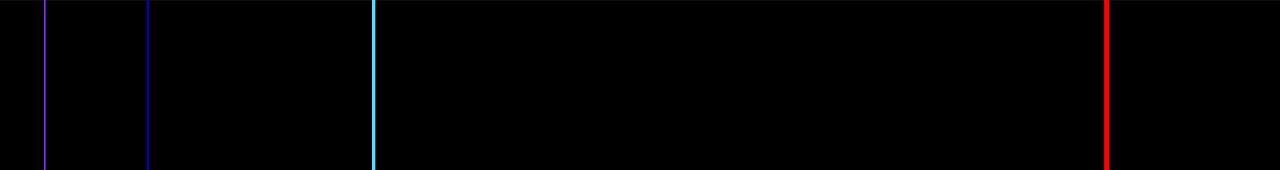
\includegraphics[width=0.70\linewidth]{images/book3/hydrogen-emission-spectrum.png}

{\small Spektrum pancaran hidrogen yang tampak: garis Balmer pada \qty{656}{nm}, \qty{486}{nm}, \qty{434}{nm} dan \qty{410}{nm}, masing-masing sebuah lompatan turun ke $n = 2$.}
\end{omfigure}

\begin{omfigure}
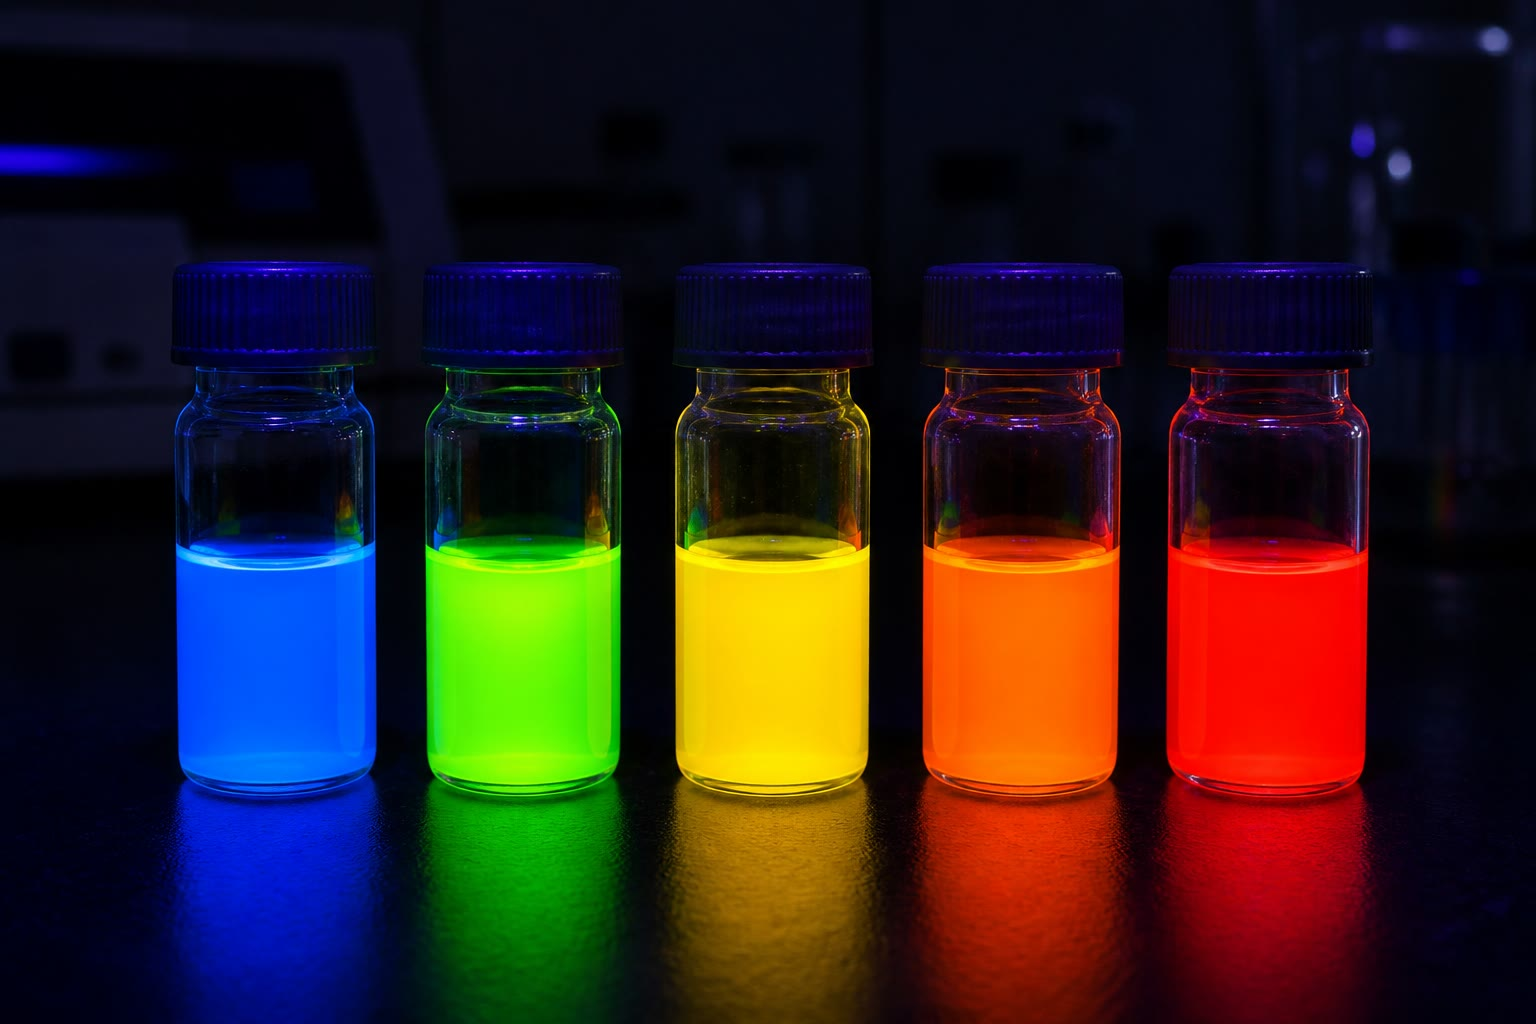
\includegraphics[width=0.60\linewidth]{images/book3/ai/b3-30-quantum-dots-vials.jpg}

{\small \omterm{ex:b1:quantum-introduction:dot}{Titik kuantum} dari satu bahan dalam botol: makin kecil nanokristalnya, makin besar energi pengurungannya dan makin biru cahayanya --- warna yang dipilih menurut ukuran.}
\end{omfigure}

\section{Soal: Spektrum hidrogen dan sebuah titik kuantum}

\begin{problem}[{Soal akhir pekan --- mengukur $h$ dengan cahaya dan sebuah
voltmeter, membangun atom hidrogen dari tiga tetapan, dan
memilih warna sebuah kristal lewat ukurannya}]
\label{pb:b1:quantum-introduction:1}
Tetapan: $h = \qty{6.626e-34}{J.s}$, $\hbar = \qty{1.055e-34}{J.s}$, $c =
\qty{3.00e8}{m/s}$, $e = \qty{1.602e-19}{C}$, $m_e = \qty{9.11e-31}{kg}$,
$1/4\pi\varepsilon_0 = \qty{8.99e9}{SI}$, $hc = \qty{1240}{eV.nm}$.

\medskip
\noindent\textbf{Bagian I --- Mengukur \omterm{thm:b1:quantum-introduction:photon}{tetapan Planck}.}
Sebuah fotokatode kalium disinari cahaya monokromatik; \omterm{prop:b1:quantum-introduction:photoelectric}{potensial
hentinya} diukur: \qty{0.30}{V} pada \qty{6.0e14}{Hz}, \qty{0.69}{V} pada
\qty{7.0e14}{Hz}, \qty{1.13}{V} pada \qty{8.0e14}{Hz}, \qty{1.50}{V} pada
\qty{9.0e14}{Hz}, \qty{2.36}{V} pada \qty{1.1e15}{Hz}.
\begin{enumerate}
  \item Lukiskanlah selnya lalu jelaskan mengapa \omterm{def:b1:dc-circuits:voltage}{tegangan} balik dapat menghentikan
        arusnya, dan apa yang diukur $eV_s$.
  \item Tuliskanlah hubungan Einstein lalu sebutkan apa yang diberikan kemiringan dan
        pintasan $V_s(\nu)$.
  \item Dari datanya (dengan pencocokan linear, atau dengan kedua titik ujungnya),
        simpulkanlah $h$; bandingkan dengan nilai yang diterima.
  \item \omterm{prop:b1:quantum-introduction:photoelectric}{Fungsi kerja} kalium dalam eV; frekuensi dan panjang gelombang
        ambangnya; dapatkah sebuah penunjuk laser merah melontarkan elektron?
  \item Intensitas lampunya dilipatduakan: apa yang terjadi pada $V_s$, pada
        arusnya? Mengapa ini tak sejalan dengan gambaran gelombang murni?
  \item Taksiran klasik: cahaya \qty{1}{\micro W/m^2} jatuh pada
        logamnya; sebuah atom menawarkan luas kira-kira \qty{1e-20}{m^2}: berapa lama
        waktu yang diperlukan untuk menumpuk \qty{2.2}{eV} pada satu atom? Apa yang
        teramati sebagai gantinya?
\end{enumerate}

\medskip
\noindent\textbf{Bagian II --- \omterm{prop:b1:quantum-introduction:hydrogen}{Atom hidrogen} Bohr.}
\begin{enumerate}[resume]
  \item Sebuah elektron pada \omterm{prop:b1:central-forces:effective}{orbit lingkaran} berjari-jari $r$ mengelilingi sebuah proton
        yang tetap: kelajuan $v(r)$ dan energi mekanisnya $E(r)$.
  \item Syarat Bohr $m_evr = n\hbar$: tunjukkan $r_n = n^2a_0$ lalu berikanlah
        $a_0 = 4\pi\varepsilon_0\hbar^2/m_ee^2$ secara numerik.
  \item $E_n = E_1/n^2$ dengan $E_1 = -m_ee^4/[2(4\pi\varepsilon_0)^2\hbar^2]$;
        nilai numeriknya dalam eV.
  \item Kelajuan pada orbit pertamanya dan nisbah $v_1/c$ (yaitu
        tetapan struktur halus $\alpha \approx 1/137$).
  \item Panjang gelombang garis $2 \to 1$ (Lyman $\alpha$), $3 \to 2$ dan
        $4 \to 2$ (Balmer H$\alpha$, H$\beta$): mana yang tampak?
  \item Tunjukkan bahwa $1/\lambda = R_H(1/n^2 - 1/p^2)$ lalu hitunglah tetapan
        Rydberg $R_H$; panjang gelombang Balmer yang terpendek.
  \item Energi ionisasi hidrogen dari \omterm{prop:b1:quantum-introduction:box}{keadaan dasarnya}; panjang gelombang
        foton yang tepat mengionkannya.
  \item De Broglie: tunjukkan bahwa keliling orbit $n$ adalah $n$
        panjang gelombang --- syarat Bohr adalah syarat \omterm{thm:b1:wave-propagation:standing}{gelombang berdiri}.
  \item Dua hal yang keliru pada modelnya, satu hal yang tepat benar,
        dan apa yang menggantikan orbitnya dalam teori lengkapnya.
\end{enumerate}

\medskip
\noindent\textbf{Bagian III --- \omterm{ex:b1:quantum-introduction:dot}{Titik kuantumnya}.}
Sebuah nanokristal CdSe berjari-jari $R$ mengurung sebuah elektron tereksitasi
(bermassa efektif $m_e^\ast = 0.13\,m_e$) dan lubang yang ditinggalkannya
($m_h^\ast = 0.45\,m_e$); energi pengurungan masing-masing dalam sebuah bola
berjari-jari $R$ adalah $h^2/8m^\ast R^2$ (diterima tanpa bukti); senjang CdSe ruahnya
$E_g = \qty{1.74}{eV}$.
\begin{enumerate}[resume]
  \item Turunkanlah energi $E_n = n^2h^2/8mL^2$ sebuah partikel dalam
        kotak satu dimensi dari syarat \omterm{thm:b1:wave-propagation:standing}{gelombang berdirinya}, lalu
        ulaslah keserupaannya dengan rumus bolanya.
  \item Energi pengurungan elektron dan lubangnya bagi
        $R = \qty{2.0}{nm}$.
  \item Energi dan panjang gelombang foton yang dipancarkan bagi $R = \qty{2.0}{nm}$,
        \qty{3.0}{nm} dan \qty{4.0}{nm}; warnanya.
  \item Jelaskanlah dalam satu kalimat mengapa titik yang lebih kecil lebih biru.
  \item Periksalah \omterm{def:b1:units-dimensions:oom}{orde besarnya} dengan asas ketakpastian:
        $\Delta p \sim \hbar/R$ bagi elektronnya pada $R = \qty{2}{nm}$, dan
        \omterm{thm:b1:work-and-energy:ke}{energi kinetik} yang tersirat darinya.
  \item Sebuah titik memancarkan \qty{1.0}{nW} pada \qty{577}{nm}: foton tiap sekon.
\end{enumerate}

\medskip
\noindent\textbf{Bagian IV --- Mencacah kuanta.}
\begin{enumerate}[resume]
  \item Foton tiap sekon dari sebuah laser \qty{1.0}{mW} pada \qty{633}{nm}.
  \item \omterm{def:b1:optical-instruments:eye}{Mata} yang telah menyesuaikan diri dengan gelap mendeteksi kilatan kira-kira $100$ foton pada
        \qty{500}{nm} yang tiba dalam \qty{0.1}{s}: daya yang bersesuaian.
  \item Sebuah antena FM menerima \qty{1.0}{pW} pada \qty{100}{MHz}: foton tiap
        sekon; adakah harapan mendeteksinya satu per satu?
  \item Ringkaslah: dari $h$, $e$, $m_e$ saja, tiga besaran dunia
        atomik mana yang dihasilkan soal ini, dan dengan
        nilai berapa?
\end{enumerate}
\end{problem}
